\section{Experimental Details}
\label{appendix:Experiement Details}
\subsection{Hardware Parameters}
\begin{figure}
    \centering
     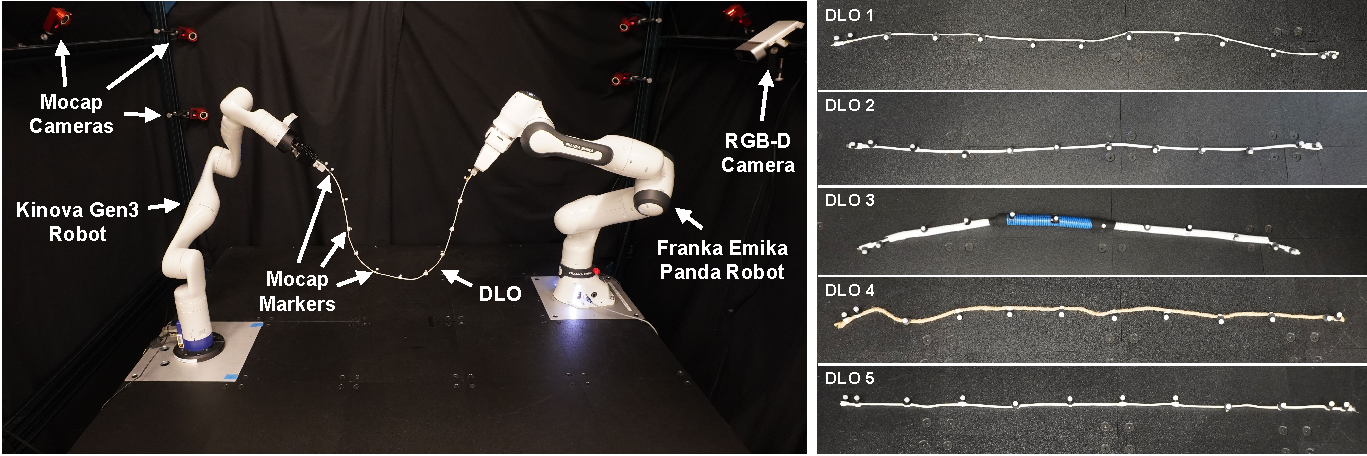
\includegraphics[width=1\textwidth]{figures/exp_set_concat.pdf}
     \caption{\textbf{Left: }An illustration of the experimental setup. \textbf{Right: }An illustration of the DLOs that are used to evaluate and compare the performance of DEFORM with various state-of-the-art DLO modeling methods. }
    \label{fig:exp_setup}
\end{figure}

We use an OptiTrack motion capture (Mocap) system to obtain the ground truth vertex locations for DLOs as depicted in Figure~\ref{fig:exp_setup}.
Spherical markers with a diameter of 7.9 mm and weight of 0.4 g, are attached to the DLOs using the OptiTrack tracking system. 
Ten Flex3 cameras capture the motion of the markers at a frequency of 100Hz, with a positional error of less than 0.3mm. 
For perception with an RGB-D camera, we use an Azure Kinect DK with a resolution of 720 x 1080 and a frequency of 30 Hz. 
Three distinct cables and two distinct ropes were constructed as shown in Figure~\ref{fig:exp_setup}.
The physical properties of each wire are outlined in Table~\ref{tab:mat_prop}. 
These properties include the length, weight, and stiffness of each DLO, as well as the number of Mocap markers attached to it.
The stiffness of each DLO is ranked on a relative scale.

\begin{table}[h]
    \centering
    \caption{Material Properties}
    \begin{tabular}{l|cccc}
        \toprule
        % & \multicolumn{3}{c}{Material Properties} \\         
        Name & Length [m] & Weight [g] & Stiffness & \makecell{ \# Mocap \\ Markers}\\ 
        \midrule
        DLO 1 & 1.152 & 34.5 & 3 & 13\\ 
        DLO 2 & 0.996 & 65.2 & 4 & 12\\
        DLO 3 & 0.998 & 96.8  & 5 & 12 \\
        DLO 4& 0.973 & 22.0 & 1 & 12\\ 
        DLO 5 & 0.988 & 19.2 & 2 & 12 \\ 
        \bottomrule
        \end{tabular}
    \label{tab:mat_prop}
\end{table}

\subsection{Software Implementation:}
All experiments were conducted in Python, on an Ubuntu 20.04 machine equipped with an AMD Ryzen PRO 5995WX CPU, 256GB RAM, and 128 cores. 
All training pipelines were built within the PyTorch training framework. 
We implement DEFORM with PyTorch and use the Levenberg-Marquardt algorithm as the solver for Theseus.
% DER's force's computational time is optimized through vectorization. 
We utilize PyTorch for training and  Numpy for non-batched prediction. 
We initialize the length and mass parameters of the DLO according to Table \ref{tab:mat_prop}. 
The other material properties are initialized randomly and learned during the training process.
We use SGD optimizer with $10^{-4}$ learning rate for training.
\subsection{Ablation Study: DLO4 and DLO5}
\label{appendix:sec:addablation1}
As a supplement for Table \ref{tab:ablation study}, the ablation study of DLO4 and DLO5 is shown in Table \ref{tab:ablation study additional DLOs}.
\begin{table}
\centering
\vspace*{-0.4cm}
\caption{Ablation Study with DLO 4 and DLO 5.}
\begin{tabular}{l|cc}
        \toprule
        & \multicolumn{2}{c}{Accuracy ($10^{-2}$m)} \\         
        Method & 4 & 5   \\
        \midrule
        DER & 1.50 & 1.65   \\ 
        W/O Residual Learning & 1.33 & 1.26    \\
        W/O System ID & 1.02 & 1.10 \\ 
        Original Inextensibility & 1.29  & 1.58   \\
        % Residual Learning & 1.81 &1.87& 1.55  \\
        % Single-Step Training & 1.82 &1.74& 1.79  \\
        DEFORM & \textbf{0.850} & \textbf{0.987}  \\
        \bottomrule
        \end{tabular}
        \vspace*{-0.3cm}
        \label{tab:ablation study additional DLOs}
\end{table}
\subsection{Ablation Study: Inextensibility 
\label{appendix:addablation2}
Enforcement with Learning and Single-step Training}
\label{sec:additional study}
\begin{table}
\centering
\caption{Additional Ablation Study.}
\begin{tabular}{l|ccc}
        \toprule
        & \multicolumn{3}{c}{Accuracy ($10^{-2}$m)} \\         
        Method & 1 & 2 & 3  \\
        \midrule
        W/O Enforcing Inextensibility with PBD & $7.7\times10^5$ & $260\times10^5$ & $310\times10^5$ \\
        Single Step Prediction Training & 1.82 &1.74& 1.79  \\ 
        % Residual Learning & 1.81 &1.87& 1.55  \\
        % Single-Step Training & 1.82 &1.74& 1.79  \\
        DEFORM & \textbf{1.01} & \textbf{0.97} & \textbf{0.77}  \\
        \bottomrule
        \end{tabular}
        \label{tab:additioanl ablation study}
\end{table}


We conducted a further ablation study on training DEFORM without the improved inextensibility enforcement and training DEFORM using only a single-step prediction as shown in Table \ref{tab:additioanl ablation study}.
When DEFORM is trained without enforcing inextensibility, simulation instability results in very high prediction loss, highlighting the importance of properly enforcing inextensibility over long time horizons.
Additionally, training DEFORM using only a single-step prediction results in lower long-term prediction accuracy compared to training DEFORM using a 100-step prediction, demonstrating the importance of DEFORM's differentiability for accurate long-term predictions.
\subsection{Effect of Number of Vertices: Accuracy and Computational Efficiency}
To further investigate the impact of vertices number on accuracy and computational efficiency, we conducted additional experiments using DLO 1. Figure \ref{fig:num_vertices} illustrates that increasing the number of vertices enhances prediction accuracy by allowing DEFORM to capture finer details due to improved resolution. 
However, this increase in detail is at the cost of reduced computational efficiency.
 In our case we chose the number of vertices to achieve optimal prediction accuracy while ensuring real-time inference capabilities at a 100Hz frequency. 
\begin{figure}[h]
    \centering
     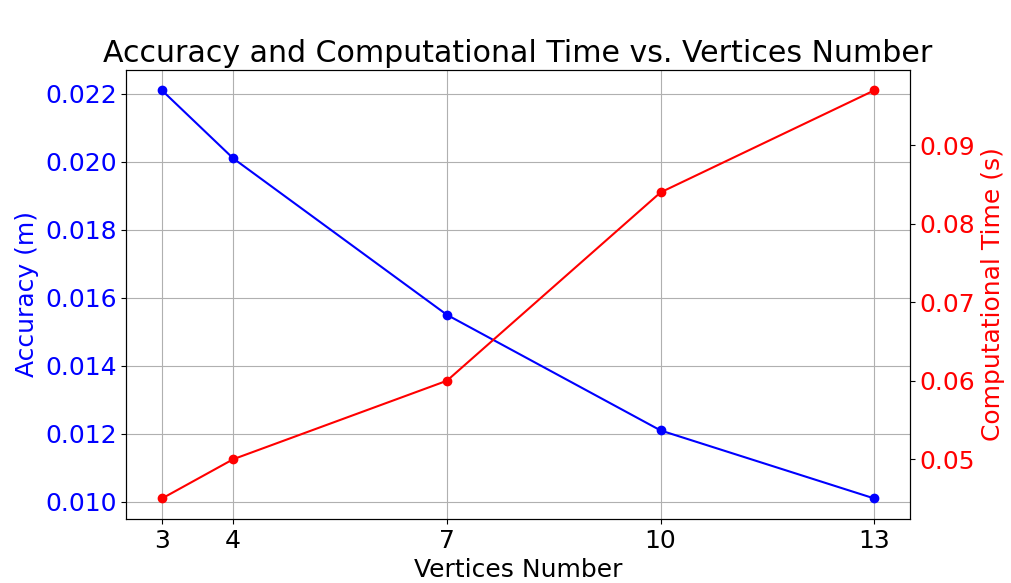
\includegraphics[width=0.6\textwidth]{figures/comptime_vertices.png}
     \caption{Accuracy and Compuational Time vs. Vertices Number}
    \label{fig:num_vertices}
\end{figure}
\subsection{ARMOUR}
\label{appendix ARMOUR}
To perform a shape matching task, we rely upon ARMOUR\cite{ARMOUR}, an optimization-based motion planning and control framework. 
The goal of the shape matching task is to use a robot arm to manipulate the DLO from an initial configuration to a predefined target configuration. 
To accomplish this goal, ARMOUR performs planning in a receding horizon fashion. 
During each planning iteration, ARMOUR selects a trajectory to follow by solving an optimization problem.
ARMOUR represents joint trajectories of the robot as polynomials, where the coefficients are considered as the decision variables of the optimization. 
One end of the rope is rigidly attached to the end effector of the robot, whose configuration can be computed by forward kinematics. 
By plugging the end effector configuration at the end of the trajectories into DEFORM, we are able to get a prediction of the rope configuration at the end of the robot motion. 
The cost function for the optimization problem to minimize is then defined as the norm distance between the predicted rope configuration and the target rope configuration. 
Joint position, velocity, and torque limits of the arm are considered as constraints of the optimization problem in ARMOUR's formulation, which ensures that the robot motion is feasible. 
The solution to this optimization problem is then the joint trajectories of the robot that manipulate the rope to approach the desired configuration. 
To command the robot to track the solution trajectories, we use the controller proposed in ARMOUR. 
This process is conducted repeatedly until the desired configuration is reached, or a planning iteration limit is reached resulting in a failure.
More details about ARMOUR's trajectory parameterization and associated closed loop controller can be found in \cite[Section IX]{ARMOUR}.
The cost function minimizes the distance between the predicted DLO configuration given a chosen robot trajectory and a target DLO configuration.
The predicted state of the DLO is computed via a DLO modeling technique.

